\chapter{Simulações e resultados}
	Neste capítulo, serão apresentados os resultados experimentais de todo o processo de obtenção do efeito de \textit{Reverb Shimmer}, bem como alguns resultados de testes de pequenos algortimos implementados no microcontrolador MSP430F5529 com seu conversor Analógico Digital de 12 bits e a comunicação I$ ^2 $C entre o $ \mu C $ e o dispositivo MCP 4725.
	
	Os experimentos ora mostrados foram realizados de forma a demonstrar toda a abordagem de aprendizagem durante o projeto. Conforme será explicado na conclusão do trabalho, posto que foi identificado, através de experimento e cálculos realizados na implementação as limitações do hardware proposto para a execução do código do efeito digital em si.

	\section{Descrição dos Experimentos}
		
		Os resultados das simulações serão divididos da seguinte ordem:
		
		\begin{enumerate}
			\item Comparativo da quantização de um sinal de aúdio com resoluções de 16 e 12 bits;
			\item Comparativo da quantização de um sinal de aúdio com resoluções de 12, 10 e 8 bits;
			\item 
		\end{enumerate}
	
		Para os experimentos acima mencionados serão utilizados os seguintes dados mostrado na tabela ():
		
		\begin{tabular}[ht!]{|c|c|}
			\hline 
			Fonte de Áudio		&	\textit{'guitar-clean16.wav'} - som de guitarra limpa\\
			\hline
			Taxa de Amostragem 	&	44100 Hz	\\
			\hline
			Número de Canais 	&	1 canal mono\\ 
			\hline

		\end{tabular}
		
		
		\begin{figure}[!ht]
			\label{fig-exp1}
			\centering
			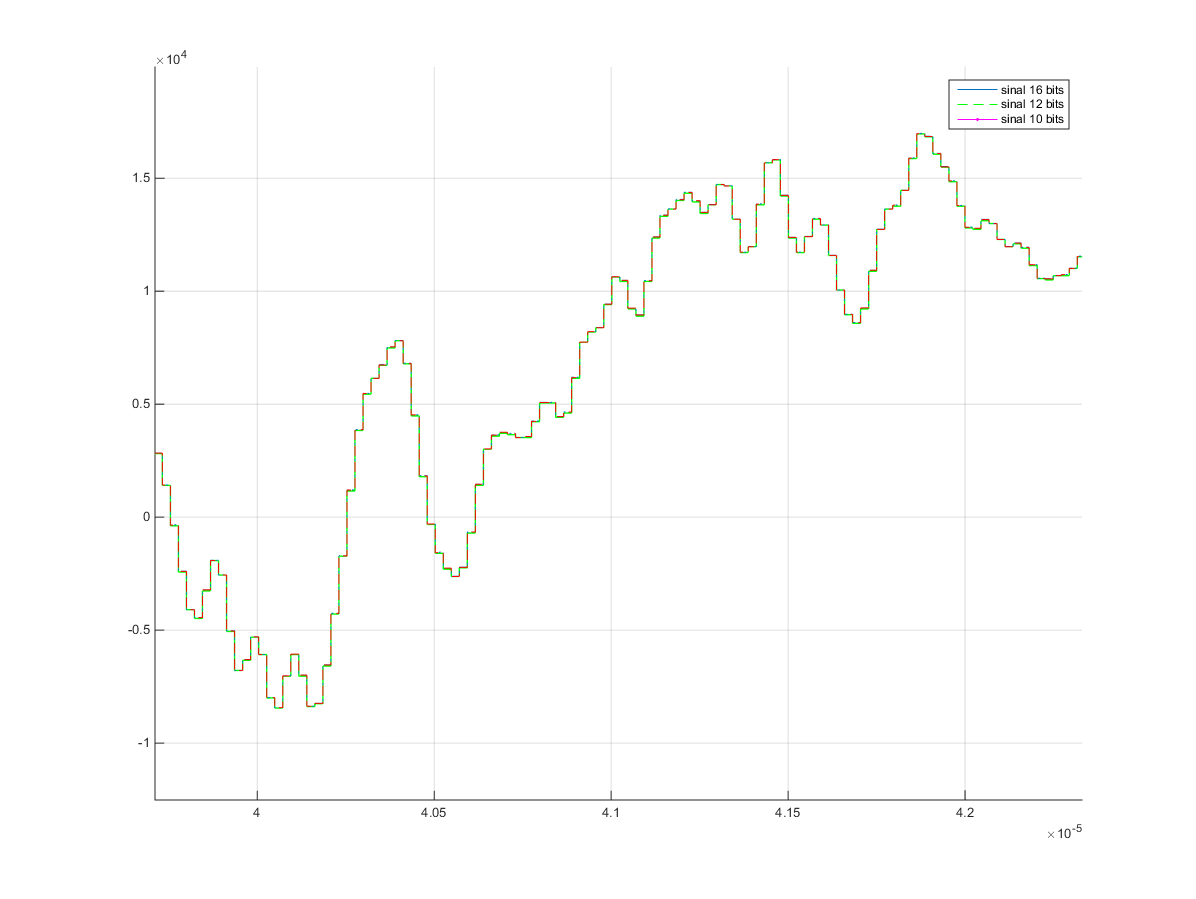
\includegraphics[scale=0.5]{./figuras/simulacoes/resolucao-audios/10-12-16-normal.png}
			\caption{Quantização do sinal de áudio em 10, 12 e 16 bits PCM}
		\end{figure}
		
		\begin{figure}[!ht]
			\label{fig-exp2}
			\centering
			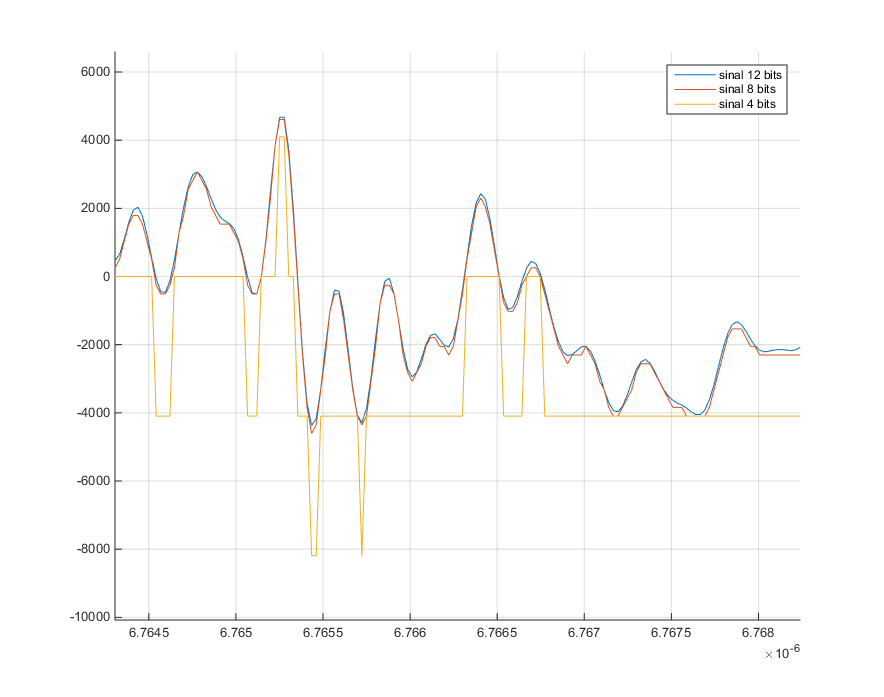
\includegraphics[scale=0.5]{./figuras/simulacoes/resolucao-audios/12-8-4-normal.png}
			\caption{Quantização do sinal de áudio em 12, 8 e 4 bits PCM}
		\end{figure}
	
		Esses resultados das figuras  são apenas a título de informações preliminares na escolha da resolução adequada para que o sinal seja tratado posteriormente no microcontrolador. Nesse caso, posto que o conversor em questão seja de 12 (doze) \textit{bits} percebe-se que não há uma perda significativa na resolução do sinal, bem como audivelmente não se percebeu grande perda de qualidade em relação ao áudio original em 16 \textit{bits}.
	
		
	
	

